%!TEX root = ../slides.tex

\section{Глиальные опухоли}

\begin{frame}
  \frametitle{Глиальные опухоли}
  %\framesubtitle{Subtitles are optional.}
  % - A title should summarize the slide in an understandable fashion
  %   for anyone how does not follow everything on the slide itself.

  \begin{itemize}
  \item \textbf{Нейроглия, или просто глия}  — совокупность вспомогательных клеток нервной ткани. 
  Составляет около 40\% объёма ЦНС. 
  \item \textbf{Астроцит}  — тип нейроглиальной 
  клетки звёздчатой формы с многочисленными отростками. Совокупность астроцитов называется астроглией.
  \item \textbf{Эпендимальные клетки} - напоминают однослойный эпителий, лежат на базальной мембране и 
  имеют кубическую или призматическую форму.
  \item\textbf{Олигодендроциты, или олигодендроглия} — вид нейроглии. Главная функция — 
  предоставлять помощь и изоляцию аксонам нейронов, находящихся в центральной нервной системе позвоночных животных.
  
  
  % 
 \end{itemize}

\end{frame}
\begin{frame}
  \begin{figure}
    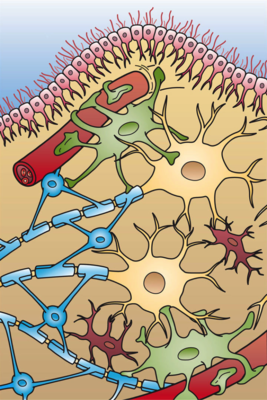
\includegraphics[scale=0.9]{glia_types.png}
    \caption{Иллюстрация четырёх типов глиальных клеток, находящихся в 
    ЦНС: эпендимный слой (светло-розовый), астроциты (зелёный), клетки микроглии (тёмно-коричневый), олигодендроциты (голубой).}
  \end{figure}
\end{frame}

\begin{frame}
  \frametitle{Глиальные опухоли}

  \begin{itemize}
  \item \textbf{Глиальная опухоль} является патологическим новообразованием, расположенным внутри мозга. 
    Она развивается из глии – вспомогательных клеток нервной ткани.
    
  \item \textbf{Астроцитома} — глиальная опухоль головного мозга, возникающая из астроцитов. 

  \item \textbf{Мультиформная глиобластома} — наиболее частая и наиболее агрессивная форма опухоли мозга,
  которая составляет до 52 \% первичных опухолей мозга и до 20 \% всех внутричерепных опухолей. 

\end{itemize}
\end{frame}

\begin{frame}
  

    \begin{figure}
      \includegraphics[scale=0.055]{Astrocytoma.jpg}
      \caption{Два ПЭТ изображения: верхнее показывает нормальный мозг, а нижнее — с астроцитомой.}
    \end{figure}
  \end{frame}


\begin{frame}
  \frametitle{Симптомы и прогноз}
  \begin{itemize}
    \item Симптомы глиомы являются переменными и зависят от расположения и размера опухоли. 
   

  \item Прогноз относительно выживаемости для данного типа опухолей ЦНС является неблагоприятным. 
  
  \end{itemize}
\end{frame}


\section{КТ/МРТ}
\begin{frame}
    \frametitle{КТ, МРТ}
    \begin{itemize}
        \item Компьютерная томография (КТ) - это специальный метод визуализации, в котором используется рентгеновское излучение. 
        \item Магнитно-резонансная томография (МРТ) - метод визуализации, основанный на резонансе атомов водорода в организме человека на магнитное поле, 
        создаваемое томографом.
    \end{itemize}
    \begin{figure}[htbp]
        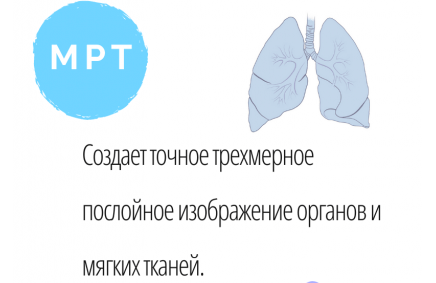
\includegraphics[scale=0.35]{mri.png}
        \hfill
        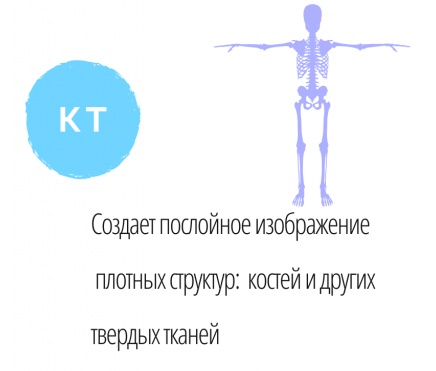
\includegraphics[scale=0.35]{ct.png}
    \end{figure}
\end{frame}


\section{ПЭТ - исследование}
\begin{frame}
    \frametitle{ПЭТ - исследование}
    \begin{itemize}
        \item Позитронно-эмиссионная томография (ПЭТ) — технология 
        визуализации, основанная на количественной и качественной 
        оценке биохимических процессов, происходящих в тканях \textit{in vivo}.
    \end{itemize}
\end{frame}
\subsection{Принцип работы ПЭТ}
\begin{frame}
    \frametitle{Принцип работы ПЭТ}
    \begin{figure}
        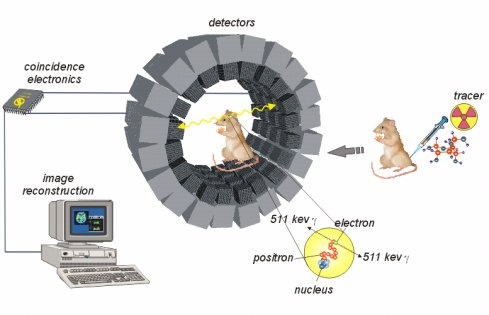
\includegraphics[scale=0.5]{pet.jpg}
    \end{figure}

    \begin{itemize}
        \item Как отличить здоровую ткань от «нездоровой»?
    \end{itemize}
    \[SUV_{\chi}=\frac{C(t)}{D/\chi}\]
\end{frame}


\begin{frame}
    \frametitle{Примеры ПЭТ - изображений}

    \begin{figure}[htbp]
        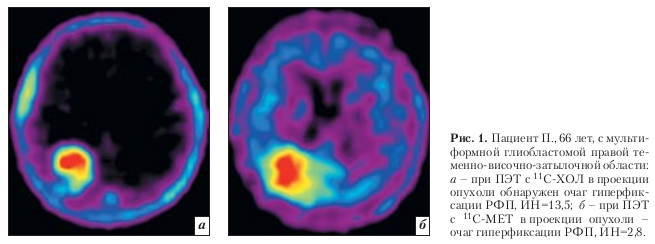
\includegraphics[scale=0.3]{pet_ex1.png}
        \hfill
        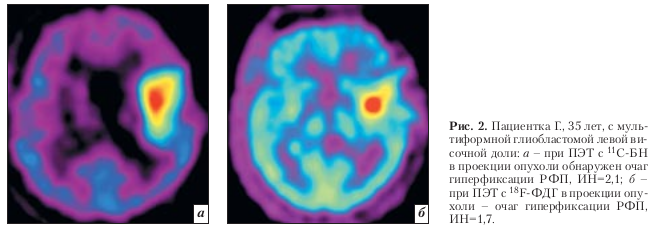
\includegraphics[scale=0.3]{pet_ex2.png}   
    \end{figure}

    \begin{figure}
        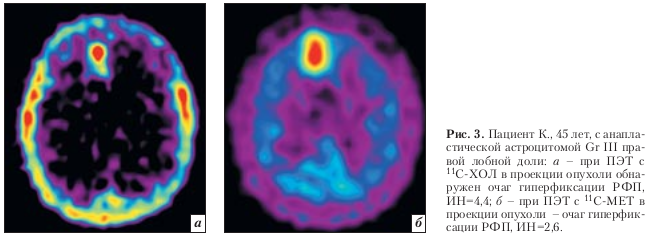
\includegraphics[scale=0.3]{pet_ex3.png}
    \end{figure}
\end{frame}

\begin{frame}
    \frametitle{ПЭТ/КТ, ПЭТ/МРТ}
    \begin{figure}
        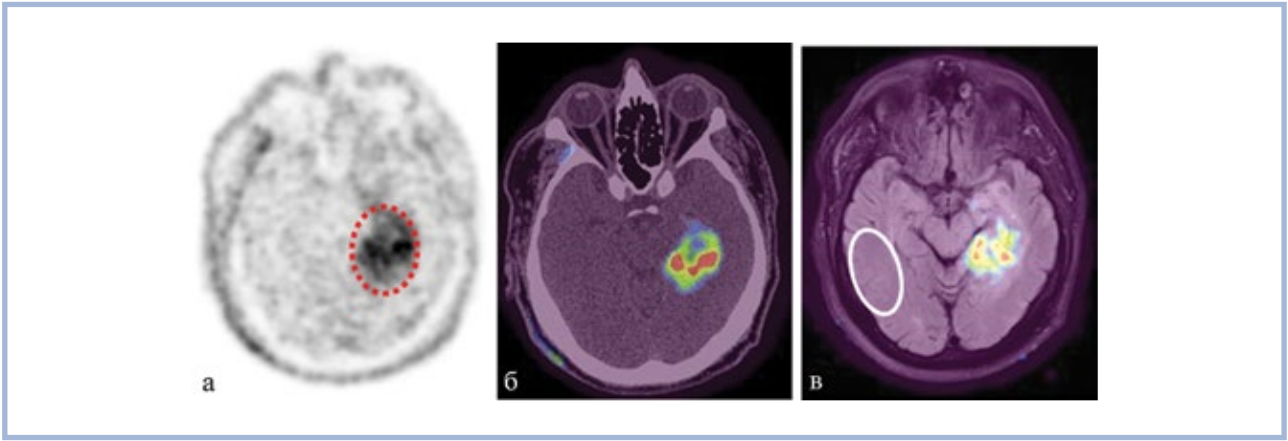
\includegraphics[scale=0.3]{pet_mri_ct.png}
    \end{figure}
\end{frame}